\documentclass[a4paper, 10.5pt, oneside, openany, uplatex]{jsarticle}

\author{山内 仁喬}
% 余白の設定.
% 参考文献:Latex2e 美文書作成入門, 14.3ページレイアウトの変更

% 行長の変更
\setlength{\textwidth}{40zw}           %全角40文字分

% 行間を制御するコマンド
\renewcommand{\baselinestretch}{0.9}

% 左マージンを変更
\setlength{\oddsidemargin}{25truemm}   % 左余白
\addtolength{\oddsidemargin}{-1truein} % 左位置デフォルトから-1inch

% 上マージンを変更
\setlength{\topmargin}{15truemm}       % 上余白
\addtolength{\topmargin}{-1truein}     % 上位置デフォルトから-1inch

% 本文領域の縦横の長さ変更
\setlength{\textheight}{242truemm}     % テキスト高さ: 297-(25+30)=242mm
\setlength{\textwidth}{160truemm}      % テキスト幅:  210-(25+25)=160mm
\setlength{\fullwidth}{\textwidth}     % ページ全体の幅


% 図・表の個数などの設定.
%% 図・表を入りやすさを制御するパラメーター
\setcounter{topnumber}{4}
\setcounter{bottomnumber}{4}
\setcounter{totalnumber}{4}
\setcounter{dbltopnumber}{3}
\setcounter{tocdepth}{1} % 項レベルまで目次に反映させるコマンド.
\renewcommand{\topfraction}{.95}
\renewcommand{\bottomfraction}{.90}
\renewcommand{\textfraction}{.05}
\renewcommand{\floatpagefraction}{.95}

% 使用するパッケージを記述.
\usepackage{amsmath} % 複雑な数式を使うときに便利
\usepackage{dcolumn}
\usepackage{color}
\usepackage{tabularx, dcolumn}
\usepackage{bm} % 数式環境内で太字を使うときに便利.
\usepackage{subcaption}  % 関連した複数の図を並べる時に使う
\usepackage[dvipdfmx]{graphicx} % 画像を挿入したり,テキストや図の拡大縮小・回転を行う.
\usepackage{verbatim} % 入力どおりの出力を行う.
\usepackage{makeidx} % 索引を作成できる.
\usepackage{dcolumn} % 表の数値を小数点で桁を揃える.
\usepackage{lscape} % 図表を90度横に倒して配置する.
\usepackage{setspace} % 行間調整.

\def\mbf#1{\mbox{\boldmath ${#1}$}}

% \newcolumntype{d}{D{+}{\,\pm\,}{4,5}}
% \newcolumntype{i}{D{+}{\,\pm\,}{-1}}
% \newcolumntype{.}{D{.}{.}{6,3}}

\begin{document}


\title{溶液中の静電相互作用}
\maketitle

\section{Debye--H\"{u}ckel理論}
\subsection{Debye--H\"{u}ckel近似の導出}
解離したイオンが極性溶媒中に溶けている場合を考える.
電場と電位の関係式, ガウスの法則の微分形はそれぞれ
\begin{align}
    \bm{E} &= - \nabla \phi
    \\
    \nabla \cdot \phi &= - \frac{4\pi\rho}{\epsilon}
\end{align}
である. これらを連立するとポアソン方程式を得る:
\begin{equation}
    \nabla^{2} \phi(r) = - \frac{4\pi\rho(r)}{\epsilon}
    \label{Eq:Poisson-Equation}
\end{equation}
ここで$\epsilon$は極性溶媒の平均誘電率である.

極性溶媒中に存在する電荷電荷を$Z_{j} e$を持つイオン$j$を考えていく.
イオンの密度$\rho_{j}(r)$はボルツマン分布に従うと仮定する. 
他のイオン$i$が作る電位を$\phi_{i}(r)$とすると, 静電エネルギーは$Z_{j}e \phi_{i}(r)$であることから, イオンの密度$\rho_{j}(r)$は
\begin{equation}
    \rho_{j}(r) =
    \rho_{j}^{(0)} \exp\left[-\beta Z_{j}e \phi_{i}(r)\right]
\end{equation}
と計算される. ここで$\beta = 1/k_{\mathrm{B}}T$は逆温度, $n_{j}^{0}$はポテンシャルがゼロの時のイオンの平均密度を表す. 
これをポアソン方程式(\ref{Eq:Poisson-Equation})に代入すると
\begin{align}
    \nabla^{2} \phi(r)
    &=
    - \frac{4\pi\rho(r)}{\epsilon}
    \notag \\
    &=
    - \frac{4\pi}{\epsilon} \sum_{j}(Z_{j} e \rho_{j})
    \notag \\
    &=
    - \frac{4\pi}{\epsilon}
    \rho_{j}^{(0)} \exp\left[-\beta Z_{j}e \phi_{i}(r)\right]
\end{align}
を得る. ここで, $\sum_{j}$はプラス電荷のイオンもマイナス電荷のイオンも足し合わせることを意味している. この方程式を解析的に解くことは困難である. そこで, $\beta Z_{j} e \phi_{i}(r) << 1$であるとする近似を行う. 近似の結果, 主要な項のみを取り出すと
\begin{equation}
    \nabla^{2} \phi(r)
    =
    \frac{4\pi}{\epsilon}
    \sum_{j} Z_{j}^{2} e^{2} \rho_{j}^{(0)} \phi_{i}(r)
\end{equation}
となる. ここで, デバイ長を
\begin{align}
    \lambda_{\mathrm{debye}} &\equiv \frac{1}{\chi} 
    \\
    \chi^{2} &\equiv 
    \frac{4\pi}{\epsilon}
    \sum_{j} Z_{j}^{2} e^{2} \rho_{j}^{(0)}
\end{align}
と定義すると, 近似したポアソン方程式は
\begin{equation}
    \nabla^{2} \phi(r) = \chi^{2} \phi_{i}(r)
\end{equation}
とかける. さらに, イオンの分布は球対称であるので$r$方向のみを考えると,
\begin{equation}
    \frac{1}{r^{2}} \frac{d}{dr}
    \left(
        r^{2}
        \frac{d\phi_{i}(r)}{dr}
    \right)
    =
    \chi^{2} \phi_{i}(r)
\end{equation}
となる. この微分方程式を解くために$u = r \phi_{i}(r)$と置くと,
\begin{equation}
    \frac{d^{2} u}{dr^{2}} = \chi^{2} u
\end{equation}
となる. この微分方程式は簡単に解ける.
無限遠において電位がゼロであるという境界条件を考慮すると, 微分方程式の解は
\begin{equation}
    u = A \exp(-\chi r)
\end{equation}
となる. したがって, 電位は
\begin{equation}
    \phi_{i}(r) = \frac{u}{r} = \frac{A}{r} \exp(-\chi r)
\end{equation}
と計算される. この式から, イオン$i$が作る電位はデバイ長$1/\chi$程度の距離で十分に減衰することが分かる. 導出の過程で, イオンの周りには他のイオンが球対称に分布していると仮定したため, デバイ長とは電位(あるいは電場)を遮蔽するようなイオンの雲の厚さだと解釈することができる.

\subsection{分子シミュレーションにおけるDebye--H\"{u}ckel型の静電相互作用}
シミュレーションでよく用いられるDebye--H\"{u}ckel型の静電相互作用の表式を見ていく.
MKSA単位系のとき, 静電相互作用は
\begin{align}
    U_{\mathrm{ele}}^{\mathrm{debye}} (r_{ij})
    &=
    \sum_{i<j}^{N}
    \frac{q_{i}q_{j}}{4\pi\epsilon_{0}\epsilon_{k}r_{ij}} e^{r_{ij}/\lambda_{\mathrm{debye}}}
    \\
    \lambda_{\mathrm{debye}}
    &=
    \left(
        \frac{\epsilon_{0}\epsilon_{k}k_{\mathrm{B}}T}{2N_{\mathrm{A}}e^{2}I}^{\frac{1}{2}}
    \right)
\end{align}
と表される.
ここで$q_{i}$は電荷, $\epsilon_{i}$は真空中での誘電率, $\epsilon_{k}$は誘電率, $N_{\mathrm{A}}$はアボガドロ数, $I$はイオン強度である.

%\subsection{Sub section}

% \subsubsection{Sub sub section}
% \begin{figure}
%  \begin{center}
%   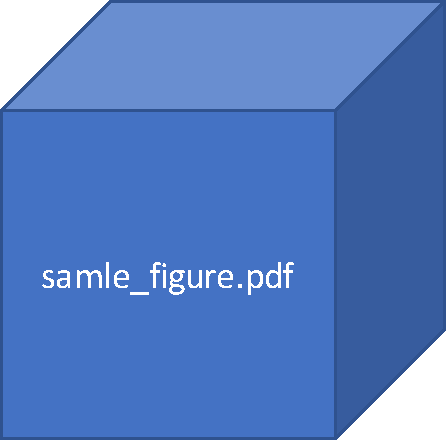
\includegraphics[width=0.5\hsize]{../figure/sample/sample_figure.pdf}
%   \caption{This is caption of sample figure.}
%   \label{Fig:Sample}
%  \end{center}
% \end{figure}

%\paragraph{Paragraph}

% \bibliographystyle{junsrt}
% \bibliography{}
\end{document}

